\documentclass[13pt]{article}
\usepackage{amsmath, amsthm, amssymb, graphicx, enumitem, esvect, tikz, graphicx}
\usetikzlibrary{automata, positioning, arrows}
\tikzset{
  ->,
  ->/.style={thick},
  every state/.style={thick, fill=gray!10},
  node distance=2.5cm,
  initial text=$ $,
}

% Language setting
% Replace `english' with e.g. `spanish' to change the document language
\usepackage[english]{babel}

% Set page size and margins
% Replace `letterpaper' with `a4paper' for UK/EU standard size
\usepackage[letterpaper,top=2cm,bottom=2cm,left=3cm,right=3cm,marginparwidth=1.75cm]{geometry}

\title{Problem Set 1}
\author{Warren Kim}

\begin{document}
\maketitle

\section*{Question 1.1}
The following are the state diagrams of two DFAs, $M_1$ and $M_2$. Answer the following questions about each of these machines.
\[\centerline{\includegraphics[scale=0.5]{hw1q1.png}}\]
\begin{enumerate}[label=(\alph*),leftmargin=*]
\item What is the start state?
\item What is the set of accepted states?
\item What sequence of states does the machine go through on input \texttt{aabb}?
\item Does the machine accept the string \texttt{aabb}?
\item Does the machine accept the string $\epsilon$?
\end{enumerate}

\subsection*{Response}
For $M_1$:
\begin{enumerate}[label=(\alph*)]
\item The start state is $q_1$.
\item The set of accepted states is $\{q_2\}$.
\item The machine goes through the sequence: $q_1, q_2, q_3, q_1, q_1$.
\item The machine does not accept the sequence \texttt{aabb}.
\item The machine does not accept the empty string $\epsilon$.
\end{enumerate}
For $M_2$:
\begin{enumerate}[label=(\alph*)]
\item The start state is $q_1$.
\item The set of accepted states is $\{q_1, q_4\}$.
\item The machine goes through the sequence: $q_1, q_1, q_1, q_2, q_4$.
\item The machine accepts the sequence \texttt{aabb}.
\item The machine accepts the empty string $\epsilon$.
\end{enumerate}

\newpage
\section*{Question 1.6}
Give state diagrams of DFAs recognizing the following languages. In all parts, the alphabet is $\{0, 1\}$.
\begin{enumerate}
\item [(b)] $\{w | w $ contains at least three $1$s$\}$
\item [(d)] $\{w | w $ has length at least $3$ and its third symbol is $0\}$
\item [(e)] $\{w | w $ starts with $0$ and has odd length, or starts with $1$ and has even length$\}$
\item [(f)] $\{w | w $ doesn't contain the substring $110\}$
\item [(h)] $\{w | w $ is any string except $11$ and $111\}$
\item [(j)] $\{w | w $ contains at least two $0$s and at most one $1\}$
\item [(k)] $\{\epsilon, 0\}$
\item [(n)] All strings except the empty string
\end{enumerate}

\subsection*{Response}
\begin{enumerate}
\item [(b)] $\{w | w $ contains at least three $1$s$\}$
  \[
    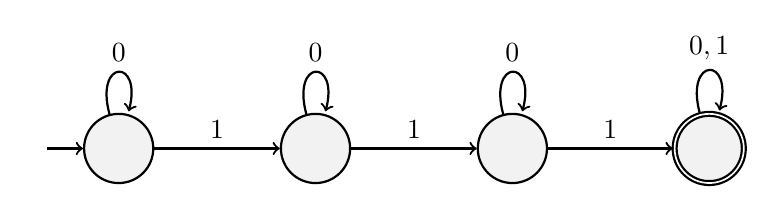
\begin{tikzpicture}
      \node[state, initial] (init) {};
      \node[state, right of=init] (q1) {};
      \node[state, right of=q1] (q2) {};
      \node[state, accepting, right of=q2] (q3) {};

      
      \draw (init) edge[->, loop above] node{$0$} (init);
      \draw (init) edge[->, above] node{$1$} (q1);

      \draw (q1) edge[->, loop above] node{$0$} (q1);
      \draw (q1) edge[->, above] node{$1$} (q2);

      \draw (q2) edge[->, loop above] node{$0$} (q2);
      \draw (q2) edge[->, above] node{$1$} (q3);

      \draw (q3) edge[->, loop above] node{$0, 1$} (q3);
    \end{tikzpicture}
  \]
\item [(d)] $\{w | w $ has length at least $3$ and its third symbol is $0\}$
  \[
    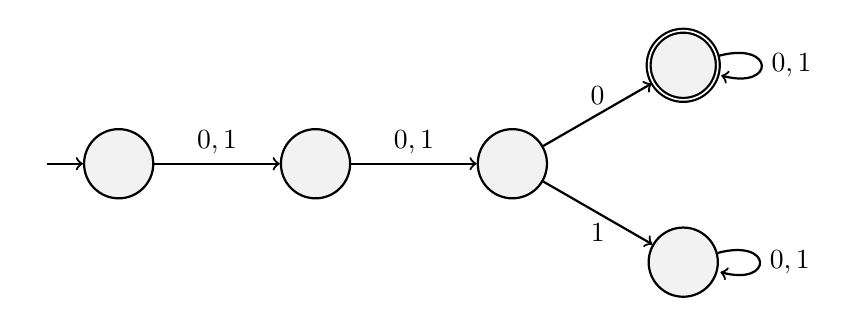
\begin{tikzpicture}
      \node[state, initial] (init) {};
      \node[state, right of=init] (q1) {};
      \node[state, right of=q1] (q2) {};
      \node[state, xshift=-0.33cm, yshift=-1.25cm, right of=q2] (sink) {};
      \node[state, accepting, xshift=-0.33cm, yshift=1.25cm, right of=q2] (q3) {};

      
      \draw (init) edge[->, above] node{$0, 1$} (q1);

      \draw (q1) edge[->, above] node{$0, 1$} (q2);

      \draw (q2) edge[->, above] node{$0$} (q3);
      \draw (q2) edge[->, below] node{$1$} (sink);

      \draw (sink) edge[->, loop right] node{$0, 1$} (sink);

      \draw (q3) edge[->, loop right] node{$0, 1$} (q3);
    \end{tikzpicture}
  \]

\item [(e)] $\{w | w $ starts with $0$ and has odd length, or starts with $1$ and has even length$\}$
  \[
    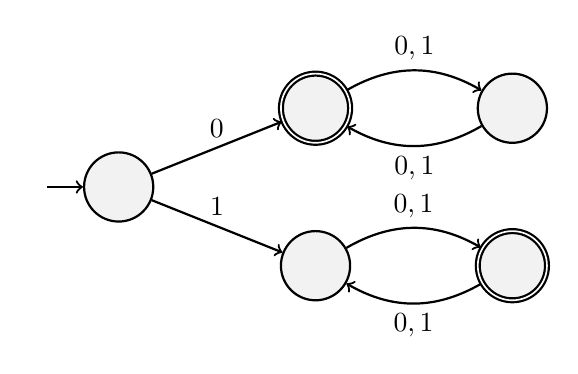
\begin{tikzpicture}
      \node[state, initial] (init) {};
      \node[state, accepting, yshift=1cm, right of=init] (q1) {};
      \node[state, right of=q1] (q2) {};

      \node[state, yshift=-1cm, right of=init] (q3) {};
      \node[state, accepting, right of=q3] (q4) {};


      \draw (init) edge[->, above] node{$0$} (q1);
      \draw (init) edge[->, above] node{$1$} (q3);

      \draw (q1) edge[->, bend left, above] node{$0, 1$} (q2);
      \draw (q3) edge[->, bend left, above] node{$0, 1$} (q4);

      \draw (q2) edge[->, bend left, below] node{$0, 1$} (q1);
      \draw (q4) edge[->, bend left, below] node{$0, 1$} (q3);      
    \end{tikzpicture}
  \]

\item [(f)] $\{w | w $ doesn't contain the substring $110\}$
    \[
    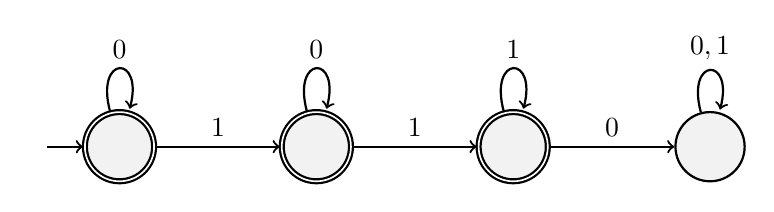
\begin{tikzpicture}
      \node[state, accepting, initial] (init) {};
      \node[state, accepting, right of=init] (q1) {};
      \node[state, accepting, right of=q1] (q2) {};
      \node[state, right of=q2] (q3) {};

      
      \draw (init) edge[->, loop above] node{$0$} (init);
      \draw (init) edge[->, above] node{$1$} (q1);

      \draw (q1) edge[->, loop above] node{$0$} (q1);
      \draw (q1) edge[->, above] node{$1$} (q2);

      \draw (q2) edge[->, loop above] node{$1$} (q2);
      \draw (q2) edge[->, above] node{$0$} (q3);

      \draw (q3) edge[->, loop above] node{$0, 1$} (q3);
    \end{tikzpicture}
  \]

\item [(h)] $\{w | w $ is any string except $11$ and $111\}$
  \[
    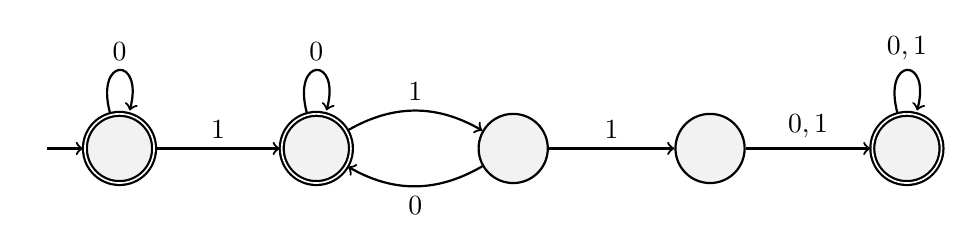
\begin{tikzpicture}
      \node[state, accepting, initial] (init) {};
      \node[state, accepting, right of=init] (q1) {};
      \node[state, right of=q1] (q2) {};
      \node[state, right of=q2] (q3) {};
      \node[state, accepting, right of=q3] (q4) {};

      
      \draw (init) edge[->, loop above] node{$0$} (init);
      \draw (init) edge[->, above] node{$1$} (q1);

      \draw (q1) edge[->, loop above] node{$0$} (q1);
      \draw (q1) edge[->, bend left, above] node{$1$} (q2);
      
      \draw (q2) edge[->, bend left, below] node{$0$} (q1);
      \draw (q2) edge[->, above] node{$1$} (q3);
      
      \draw (q3) edge[->, above] node{$0, 1$} (q4);

      \draw (q4) edge[->, loop above] node{$0, 1$} (q4);
    \end{tikzpicture}
  \]

\item [(j)] $\{w | w $ contains at least two $0$s and at most one $1\}$
  \[
    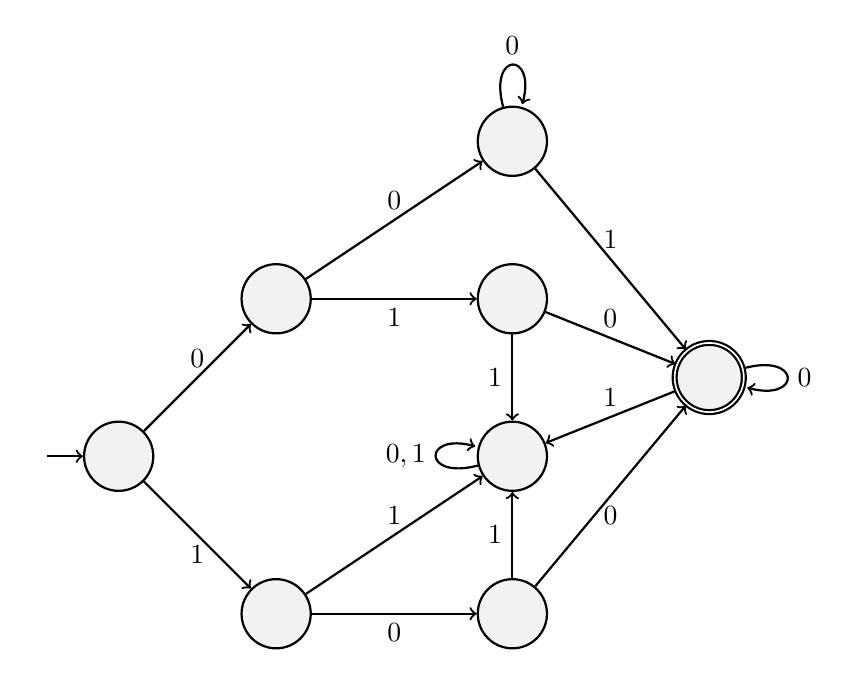
\begin{tikzpicture}
      \node[state, initial] (init) {};
      \node[state, xshift=2cm, yshift=2cm] (t1) {};
      \node[state, xshift=5cm, yshift=2cm] (t2) {};
      \node[state, xshift=5cm, yshift=4cm] (t3) {};

      \node[state, xshift=2cm, yshift=-2cm] (b1) {};
      \node[state, xshift=5cm, yshift=-2cm] (b2) {};

      \node[state, xshift=5cm] (sink) {};

      \node[state, accepting, xshift=7.5cm, yshift=1cm] (goal) {};
      

      \draw (init) edge[->, above] node{$0$} (t1);
      \draw (init) edge[->, below] node{$1$} (b1);

      \draw (t1) edge[->, below] node{$1$} (t2);
      \draw (t1) edge[->, above] node{$0$} (t3);

      \draw (t2) edge[->, above] node{$0$} (goal);
      \draw (t2) edge[->, left] node{$1$} (sink);

      \draw (t3) edge[->, above] node{$1$} (goal);
      \draw (t3) edge[->, loop above] node{$0$} (t3);

      \draw (b1) edge[->, above] node{$1$} (sink);
      \draw (b1) edge[->, below] node{$0$} (b2);

      \draw (b2) edge[->, below] node{$0$} (goal);
      \draw (b2) edge[->, left] node{$1$} (sink);

      \draw (sink) edge[->, loop left] node{$0, 1$} (sink);

      \draw (goal) edge[->, loop right] node{$0$} (goal);
      \draw (goal) edge[->, above] node{$1$} (sink);
    \end{tikzpicture}
  \]
\item [(k)] $\{\epsilon, 0\}$
  \[
    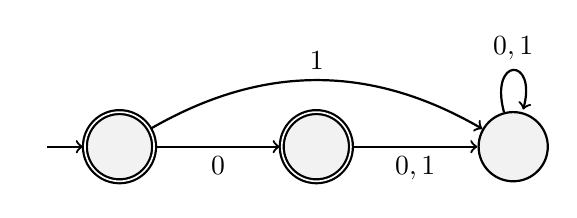
\begin{tikzpicture}
      \node[state, accepting, initial] (init) {};
      \node[state, accepting, right of=init] (q1) {};
      \node[state, right of=q1] (sink) {};

      
      \draw (init) edge[->, below] node{$0$} (q1);
      \draw (init) edge[->, bend left, above] node{$1$} (sink);

      \draw (q1) edge[->, below] node{$0, 1$} (sink);
      
      \draw (sink) edge[->, loop above] node{$0, 1$} (sink);
    \end{tikzpicture}
  \]
  
\item [(n)] All strings except the empty string
  \[
    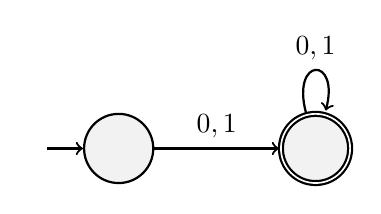
\begin{tikzpicture}
      \node[state, initial] (init) {};
      \node[state, accepting, right of=init] (q1) {};

      \draw (init) edge[->, above] node{$0, 1$} (q1);

      \draw (q1) edge[->, loop above] node{$0, 1$} (q1);
    \end{tikzpicture}
  \]

\end{enumerate}

\end{document}

%%% Local Variables:
%%% mode: latex
%%% TeX-master: t
%%% End:
